\documentclass[letterpaper]{article}
\usepackage[margin=1in]{geometry}
\usepackage[utf8]{inputenc}
\usepackage{textcomp}
\usepackage{amssymb}
\usepackage{natbib}
\usepackage{graphicx}
\usepackage{gensymb}
\usepackage{amsthm, amsmath, mathtools}
\usepackage[dvipsnames]{xcolor}
\usepackage{enumerate}
\usepackage{mdframed}
\usepackage[most]{tcolorbox}
\usepackage{csquotes}
% https://tex.stackexchange.com/questions/13506/how-to-continue-the-framed-text-box-on-multiple-pages

\tcbuselibrary{theorems}

\newcommand{\R}{\mathbb{R}}
\newcommand{\Z}{\mathbb{Z}}
\newcommand{\N}{\mathbb{N}}
\newcommand{\Q}{\mathbb{Q}}
\newcommand{\C}{\mathbb{C}}
\newcommand{\code}[1]{\texttt{#1}}
\newcommand{\mdiamond}{$\diamondsuit$}
\newcommand{\PowerSet}{\mathcal{P}}
\newcommand{\Mod}[1]{\ (\mathrm{mod}\ #1)}
\DeclareMathOperator{\lcm}{lcm}

%\newtheorem*{theorem}{Theorem}
%\newtheorem*{definition}{Definition}
%\newtheorem*{corollary}{Corollary}
%\newtheorem*{lemma}{Lemma}
\newtheorem*{proposition}{Proposition}


\newtcbtheorem[number within=section]{theorem}{Theorem}
{colback=green!5,colframe=green!35!black,fonttitle=\bfseries}{th}

\newtcbtheorem[number within=section]{definition}{Definition}
{colback=blue!5,colframe=blue!35!black,fonttitle=\bfseries}{def}

\newtcbtheorem[number within=section]{corollary}{Corollary}
{colback=yellow!5,colframe=yellow!35!black,fonttitle=\bfseries}{cor}

\newtcbtheorem[number within=section]{lemma}{Lemma}
{colback=red!5,colframe=red!35!black,fonttitle=\bfseries}{lem}

\newtcbtheorem[number within=section]{example}{Example}
{colback=white!5,colframe=white!35!black,fonttitle=\bfseries}{def}

\newtcbtheorem[number within=section]{note}{Important Note}{
        enhanced,
        sharp corners,
        attach boxed title to top left={
            xshift=-1mm,
            yshift=-5mm,
            yshifttext=-1mm
        },
        top=1.5em,
        colback=white,
        colframe=black,
        fonttitle=\bfseries,
        boxed title style={
            sharp corners,
            size=small,
            colback=red!75!black,
            colframe=red!75!black,
        } 
    }{impnote}
\usepackage[utf8]{inputenc}
\usepackage[english]{babel}
\usepackage{fancyhdr}
\usepackage[hidelinks]{hyperref}

\pagestyle{fancy}
\fancyhf{}
\rhead{CSE 131}
\chead{Friday, May 26, 2023}
\lhead{Lecture 24}
\rfoot{\thepage}

\setlength{\parindent}{0pt}

\begin{document}

\section{Optimization (Continued)}
\subsection{Intermediate Representation}
\subsubsection{Rust AST}
Given what we've just discussed, the Rust representation of A-Normal Form and ANF-Restricted Form might look something like 
\begin{verbatim}
    pub enum AVal {
        Num(i32),
        True,
        False,
        Id(String),
    }

    pub enum AExpr {
        Plus(Box<AVal>, Box<AVal>),
        Eq(Box<AVal>, Box<AVal>),
        Lt(Box<AVal>, Box<AVal>),
        Print(Box<AVal>),
        Set(String, Box<AVal>),
        Call1(String, Box<AVal>),
        Call2(String, Box<AVal>, Box<AVal>),
        Pair(Box<AVal>, Box<AVal>),
        Fst(Box<AVal>),
        Snd(Box<AVal>),
        Break(Box<AVal>),
        Loop(Box<ABlock>),
        If(Box<AVal>, Box<ABlock>, Box<ABlock>),
        Val(Box<AVal>),
    }

    pub enum ABlock {
        Let(String, Box<AExpr>, Box<ABlock>),
        Block(Vec<ABlock>),
        Op(Box<AExpr>),
    }\end{verbatim}

\subsubsection{A Problem With Loops}
Consider the following function:
\begin{verbatim}
    (fun (range low high)
        (let (n high)
            (let (lst nil)
                (loop
                    (if (= n low) (break lst)
                        (block
                            (set! n (+ n -1))
                            (set! lst (pair n lst)))
                    )
                )
            )
        )
    )
\end{verbatim}
Converting the above function, which is written in A-Normal Form, to ANF-Restricted Form, yields:
\begin{verbatim}
    (fun (range low high)
        (let (n high)
            (let (lst nil)
                (loop
                    (let (%t_0 (= n low))
                        (if %t_0 (break lst)
                            (block
                                (let (%t_1 (+ n -1)) (set! n %t_1))
                                (let (%t_2 (pair n lst)) (set! lst %t_2)))
                        )
                    )
                )
            )
        )
    )\end{verbatim}
Note that the \verb|%| identifiers are just the convention we're using for temporaries. Let's now consider all interfering variables, which we can do by considering all variables inside-out. 
\begin{verbatim}
    (fun (range low high)
        (let (n high)           ; low, high
            (let (lst nil)                  ; n, low
                (loop
                    (let (%t_0 (= n low))           ; lst, n, low, t_0
                        (if %t_0 (break lst)        ; n, lst, t_0
                            (block
                                (let (%t_1 (+ n -1)) (set! n %t_1))         ; t_1, n, lst
                                (let (%t_2 (pair n lst)) (set! lst %t_2)))  ; t_2, lst, n
                        )
                    )
                )
            )
        )
    )\end{verbatim}
Notice that we end up with the set of variables $\{\code{n}, \code{low}, \code{lst}, \verb|t_0|, \verb|t_1|, \verb|t_2|, \code{high}\}$. A graph representing this would look like 
\begin{center}
    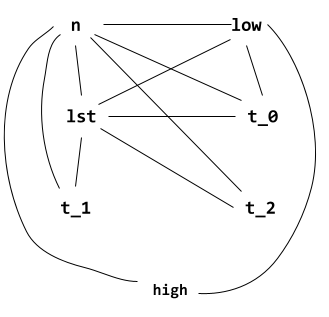
\includegraphics[scale=0.6]{../assets/loc_pt2.png}
\end{center}

\begin{mdframed}
    (Exercise.) How would the graph change if we swapped the order of the \code{set!} lines?

    \begin{mdframed}
        \underline{Suggestion:} Because the last use of \code{lst} would be in the first \code{set!} instead of the last line, there wouldn't be an edge between \code{lst} and \code{t\_1}. 

        \bigskip 

        But, one thing to keep in mind is that the \code{set!} is in a loop. So, \code{lst} needs to be in scope for the remainder of the block statement. Otherwise, a temporary could be assigned to the same register that was being used for \code{lst}. 
    \end{mdframed}
\end{mdframed}
\textbf{Remarks:}
\begin{itemize}
    \item Remember that our algorithm just went from the end to beginning, but now we need to consider what identifiers have been defined outside of the loop. 

    \item The issue with loops is that you have implicit backedges from the last expression in the loop to the beginning of the loop. We don't have names associated with these loops, which makes things difficult since we have names in the first place so we know where everything is. 
\end{itemize}

\subsubsection{A Rewrite of the Grammar}
How do we rewrite our grammar to account for loops? 
\begin{verbatim}
    pub enum Val {
        Num(i32),
        True,
        False,
        Id(String),
    }


    pub enum Expr {
        Plus(Box<Val>, Box<Val>),
        Eq(Box<Val>, Box<Val>),
        Lt(Box<Val>, Box<Val>),
        Print(Box<Val>),
        Call1(String, Box<Val>),
        Call2(String, Box<Val>, Box<Val>),
        Pair(Box<Val>, Box<Val>),
        Fst(Box<Val>),
        Snd(Box<Val>),
        Val(Box<Val>),
    }


    pub enum Step {
        Label(String),
        If(Box<Val>, String, String)
        Goto(String),
        Do(Expr),
        Set(String, Expr)
    }


    pub struct Block {
        pub steps: Vec<Step>,
    }\end{verbatim}
Some things to notice here: 
\begin{itemize}
    \item Rather than expressing our program as loops with breaks, we'll express them as labels and gotos. 
    \item In the \code{if}-condition, the first \code{String} is the label to jump to if the condition is true; the last \code{String} is the label to jump to if the condition is false. 
    \item So, whereas ANF is about scope and temporary variables, this is about control flow. Essentially, we're iteratively getting closer to assembly.
\end{itemize}
Here, we introduce the concept of \textbf{intermediate representation}. With the above new representation, we have the following intermediate representation:
\begin{verbatim}
    range(low,high) {
        n <- high
        lst <- nil
       loop_0:
        %t_0 <- n == low
        if %t_0 thn_3 els_4
       thn_3:
        rax <- lst
        goto end_1
        goto ifend_2
       els_4:
        %t_1 <- pair(n, lst)
        lst <- %t_1
        %t_2 <- n + -1
        n <- %t_2
        rax <- n
        goto ifend_2
       ifend_2:
        goto loop_0
       end_1:
        return rax
    }\end{verbatim}
Note that this is the compiled output of the \code{range} function, not in x86\_64. Some things to note: 
\begin{itemize}
    \item There's no nesting of expressions anymore. There's no notion of labels being inside other labels. 
    \item Lots of IRs have support for functions (including things like function scope, blocks within functions, etc.), but leave the actual calling convention to the language. 
    \item The pipeline we would have is that surface syntax turns into ANF, and then ANF turns into IR. It's possible to do everything in one pass, but it's easier to do it in two passes.
    \item In this example of \code{range}, \code{rax} is now our designated answer variable, and we expect all lines before the \code{return rax} line to store the answer into \code{rax} (similar to what our compiler does right now).
\end{itemize}
With that said, running through the IR representation from last to start, the variables in use are: 
\begin{verbatim}
    range(low,high) {           ; {}
        n <- high               ; n
        lst <- nil              ; n, lst 
       loop_0:                  ; n, lst
        %t_0 <- n == low        ; t_0, n, lst 
        if %t_0 thn_3 els_4     ; t_0, n, lst  
       thn_3:                   ; lst 
        rax <- lst              ; rax, lst 
        goto end_1              ; rax 
        goto ifend_2            ; <empty for now>
       els_4:                   ; n, lst, t_1
        %t_1 <- pair(n, lst)    ; n, lst, t_1
        lst <- %t_1             ; lst, n, t_1
        %t_2 <- n + -1          ; t_2, n 
        n <- %t_2               ; t_2, n 
        rax <- n                ; n, rax 
        goto ifend_2            ; <empty for now>
       ifend_2:                 ; <empty for now>
        goto loop_0             ; <empty for now>
       end_1:                   ; rax 
        return rax              ; rax
    }\end{verbatim}
Any time you reach a \code{goto}, any variables that are used at the jump target are copied over to the \code{goto}. In any case, we should not use this information to construct the graph needed to figure out how many registers we need to allocate. In particular, at these three instructions,
\begin{verbatim}
    %t_2 <- n + -1          ; t_2, n 
    n <- %t_2               ; t_2, n 
    rax <- n                ; n, rax \end{verbatim}
there's no edge between \code{lst} and \code{t\_2}. This means that we could potentially store \code{lst} and \code{t\_2} into the same register, losing a possible important value. So, we need to run this same algorithm over and over until none of the sets change (i.e., when saturation occurs). Running through the algorithm again gives us: 
\begin{verbatim}
    range(low,high) {           ; {}                ; 
        n <- high               ; n                 ; 
        lst <- nil              ; n, lst            ; 
       loop_0:                  ; n, lst            ; 
        %t_0 <- n == low        ; t_0, n, lst       ; 
        if %t_0 thn_3 els_4     ; t_0, n, lst       ; 
       thn_3:                   ; lst               ; 
        rax <- lst              ; rax, lst          ;
        goto end_1              ; rax               ; 
        goto ifend_2            ; <empty for now>   ; n, lst
       els_4:                   ; n, lst, t_1       ; 
        %t_1 <- pair(n, lst)    ; n, lst, t_1       ; 
        lst <- %t_1             ; lst, n, t_1       ; 
        %t_2 <- n + -1          ; t_2, n            ; lst 
        n <- %t_2               ; t_2, n            ; lst 
        rax <- n                ; n, rax            ; lst
        goto ifend_2            ; <empty for now>   ; n, lst
       ifend_2:                 ; <empty for now>   ; n, lst
        goto loop_0             ; <empty for now>   ; n, lst
       end_1:                   ; rax               ; 
        return rax              ; rax               ; 
    }\end{verbatim}
Note that the last column are the variables \emph{added} to the variables mentioned in the second columns. Anyways, after running this algorithm again, we reach saturation -- we don't find any additional variables that need to be added. This gives us a complete graph that we can use to determine what registers can be allocated.


\end{document}